\documentclass[11pt, a4paper]{article}
\usepackage[a4paper, total={6in, 9.5in}]{geometry}

\title{\textbf{\Huge Gravitational Wave Physics and LIGO}}


\usepackage{amsmath, tensor, gensymb, graphicx, hyperref, authblk, amsfonts, amssymb, verbatim}
\usepackage[T1]{fontenc}
\usepackage[utf8]{inputenc}
\usepackage[english]{babel}
\usepackage[sorting = none]{biblatex}

\addbibresource{bibliography.bib}

\author[1]{Sagar JC}
\author[1]{Aditya Srivatsa}
\author[1]{Ajith U Shanbhag}
\author[2]{Kushal J}
\author[3]{Hardik Medhi}
\author[4]{Bhavya Goradia}
\author[5]{Kshitija Kshirsagar}
\author[6]{Tasmi Memon}
\author[7]{Samrudhi R Kanjarpane}
\author[8]{Ajay Atwal}
\author[9]{Tanay}


\affil[1]{St. Joseph's College, Bengaluru}
\affil[2]{Christ Junior College, bengaluru}
\affil[3]{REVA University, Bengaluru}
\affil[4]{KJ Somaiya College of Engineering, Mumbai}
\affil[5]{Institute of Science, Nagpur}
\affil[6]{Maharaja Sayajirao University, Vadodara}
\affil[7]{Poornaprajna College, Udupi}
\affil[8]{University of Hyderabad}
\affil[9]{Mumbai University, Mumbai}


\renewcommand\Authands{and }

\date{\today}

\begin{document}
\maketitle

\section*{Acknowledgement}
A special thanks to Naxxatra Science for giving us the opportunity to write a collaborative review paper. We would like to express our gratitude to Ms. Sitara Srinivasan, owner of Naxxatra Science, Mr. Vikranth Pulamathi and Mr. Jishnu P Das for teaching us \LaTeX.

\pagebreak
\begin{center}
    \section*{Abstract}
\end{center}

Abstract here

\pagebreak

\providecommand{\keywords}[1]
{
  \small	
  \textbf{\textit{Keywords---}} #1
}

\keywords{General Relativity, Space time, Tensors, indices, Field equations, Wave equation, Polarization, Energy Flux, Doppler effect, Inverse square law, Inspiral mechanism, Black holes, Neutron stars, Pulsars, Add key words here relating to ur topic}
\pagebreak

\tableofcontents

\section{Introduction}
Write small paragraph about general relativity

Write small paragraph about Space-time
write who al worked in the field of general relativity and gravitational waves 
write a small intro for gravitational waves

\pagebreak

\section{Linearized theory of Gravitational waves}
Linearized theory of Gravitational waves is a basic understanding of gravitational waves based on an assumption that any perturbation in space-time can be approximated to a linear factor whose degree is One. This simplifies the calculations a lot. And more over since the sources of gravitational waves are very far away, the effects they produce here on earth will be very small. So we can neglect the higher degree of perturbation and linearize it to the first degree. \\

Einstein's field equations are a set of ten Tensor equations which describe gravity as a curvature in space-time. And one among them is: 
\begin{equation}
    G_{\mu\nu}= \frac{8 \pi  G}{c^{4}}  T_{\mu\nu}
\end{equation}
This is a tensor equation which describes gravity in form of Einstein's tensor, $G_{\mu\nu}$ which is directly dependent on the geometry of space-time which is altered by the stress-energy tensor $T_{\mu\nu}$. Another field equation that relates the geometry or curvature of space-time to stress-energy tensor is 

\begin{equation}
    R_{\mu\nu}-\frac{1}{2}g_{\mu\nu}R=\frac{8\pi G}{c^{4}}T_{\mu\nu}
\end{equation}
where $R_{\mu\nu}$ is the Riemann tensor which describes the curvature of space-time, $R$ is the scalar curvature and $g_{\mu\nu}$ is the gravitational field tensor. Any change in matter distribution will be recorded in in $T_{\mu\nu}$. So if $T_{\mu\nu}$ changes then according to equation 2, gravitational field tensor $g_{\mu\nu}$ also has to change. If $h_{\mu\nu}$ is the perturbation induced in space-time then the new gravitational field tensor $\tilde{g}_{\mu\nu}$ is given by \cite{Kokkotas_2008}

\begin{equation}
    \tilde{g}_{\mu\nu} = g_{\mu\nu} + h_{\mu\nu}
\end{equation}

\noindent To get the new gravitational field, field equation should be solved for $\tilde{g}_{\mu\nu}$ which gives 

\begin{equation}
    \tilde{h}_{\mu\nu} = h_{\mu\nu} - \frac{1}{2} \, \eta_{\mu\nu} \, h^{\alpha}_{\alpha}
\end{equation}
 where $\eta_{\mu\nu}$ is the gravity where space is flat i.e. $\eta_{\mu\nu} = g_{\mu\nu}$ and $h^{\alpha}_{\alpha}$ is summed for all spatial coordinates i.e. $\alpha$ takes values $(1,2,3) $ which corresponds to $(x,y,z)$. The admitted solutions for this variations in space time $\tilde{h}_{\mu\nu}$ has solution in the form of 
 
 \begin{equation}
     \tilde{h}_{\mu\nu} = A^{\mu\nu}\, e^{ik_{\alpha}x^{\alpha}}
 \end{equation}
 
 \noindent This is a 3D wave equation where $A^{\mu\nu}$ is the Amplitude tensor, $i = \sqrt{-1} $, $k_{\alpha} = (k_{x},k_{y},k_{z})$ is the wave vector and $x^{\alpha} = (x^{1},x^{2},x^{2}) = (x,y,z)$ is the position vector.
 \\
 
 Thus we can say that when ever a body causes disturbances in curvature of space-time, these travel through space in form of waves whose speed is equal to the speed of light.  
 
\begin{figure}[h]
     \centering
     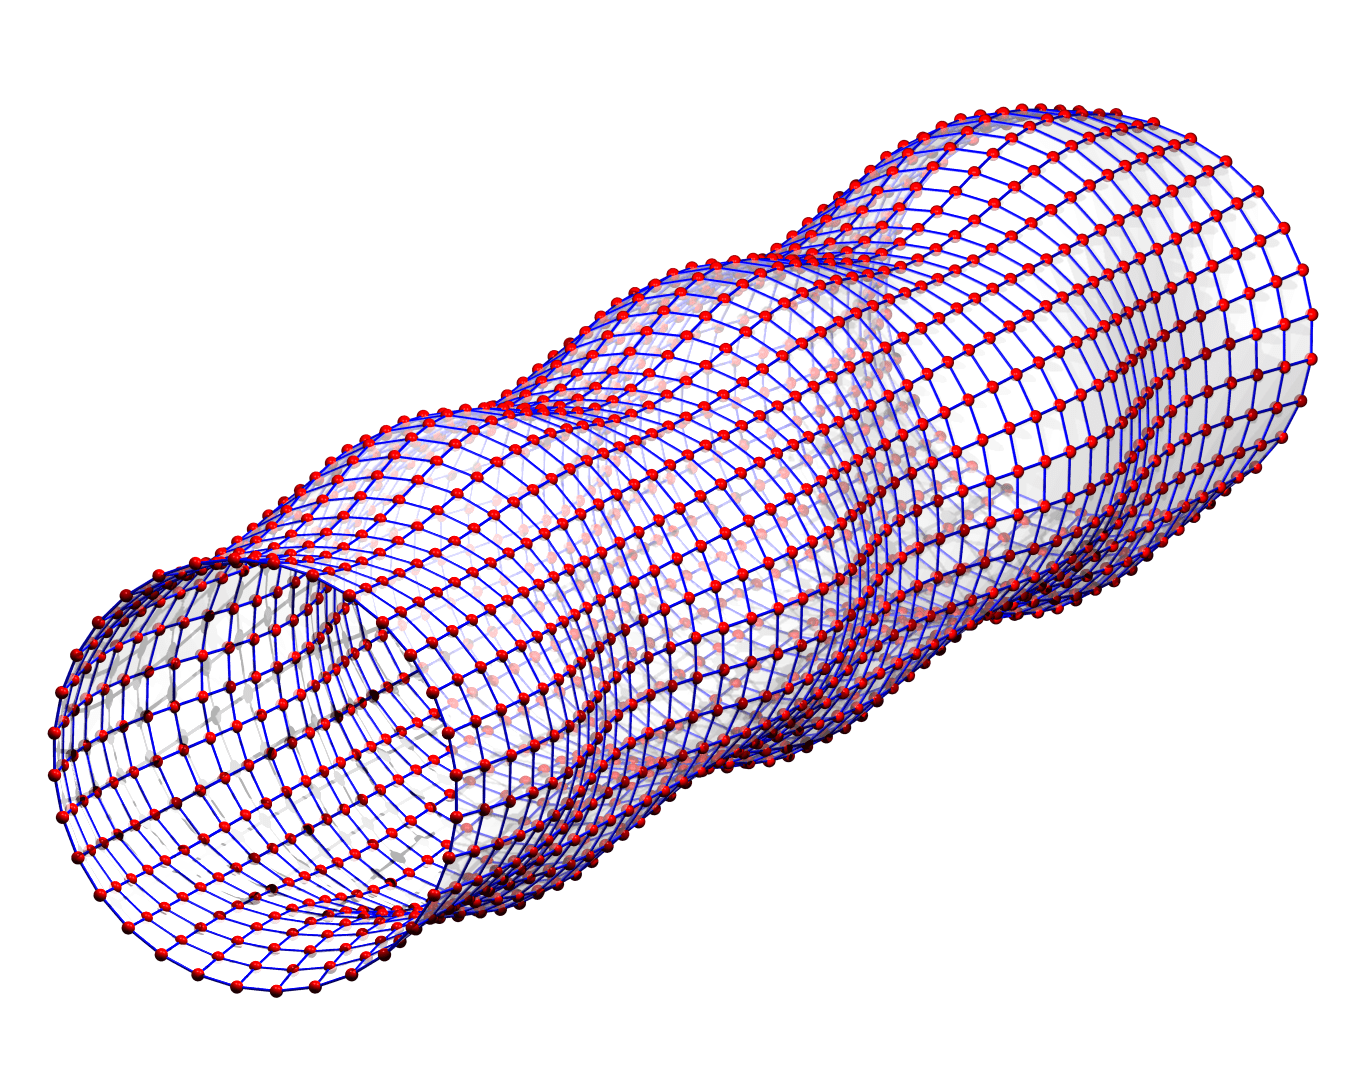
\includegraphics[scale=0.13]{images.tex/gw_representation.png}
     \caption{This is a computer simulated image that shows Gravitational wave as a 3D wave.\\ 
     Source:- \href{https://www.universetoday.com/127255/gravitational-waves-101/}{Universetoday.com}}
 \end{figure}


\section{Properties of Gravitational waves}
Now we shall see the properties of these gravitational waves. like any other waves, even gravitational waves have frequency, wavelength, speed which is speed of light, etc. These properties depend on the source of gravitational waves. 
\subsection{Polarization of Gravitational waves}


Gravitational waves can also be. Since they are three dimensional waves their polarization can be restricted to two forms where the the amplitude tensor $A^{\mu\nu}$ has two forms $A^{\mu\nu}_{+}$ and $A^{\mu\nu}_{\times}$ which are orthogonal to each other. They can be represented as 

\begin{equation}
    A^{\mu\nu}_{+} = h_{+}\, \varepsilon^{\mu\nu}_{+}
\end{equation}

\begin{equation}
    A^{\mu\nu}_{\times} = h_{\times} \,\varepsilon^{\mu\nu}_{\times}
\end{equation}

\noindent where $\varepsilon^{\mu\nu}_{+}$ and $\varepsilon^{\mu\nu}_{\times}$ are unit polarization tensors.

\begin{equation}
\varepsilon^{\mu\nu}_{+} =
\begin{bmatrix}
0 & 0 & 0 & 0 \\
0 & +1 & 0 & 0 \\
0 & 0 & -1 & 0 \\
0 & 0 & 0 & 0 \\
\end{bmatrix}
\end{equation}
\\
\begin{equation}
\varepsilon^{\mu\nu}_{\times} =
\begin{bmatrix}
0 & 0 & 0 & 0 \\
0 & 0 & +1 & 0 \\
0 & +1 & 0 & 0 \\
0 & 0 & 0 & 0 \\
\end{bmatrix}
\end{equation}

\noindent In general relativity any tensor with indices $\mu\nu$ is a rank 2 tensor with 4 rows and 4 columns where each index can take values of space time coordinates which are $(t,x,y,z)$ , and position of each element is associated with any two coordinates. Thus in such tensors, the positions of elements are associated with space-time as follows:

\begin{equation*}
    \begin{bmatrix}
    tt & tx & ty & tz \\
    xt & xx & xy & xz \\
    yt & yx & yy & yz \\
    zt & zx & zy & zz \\
    \end{bmatrix}
\end{equation*}

\noindent So when we compare the unit polarization tensors $\varepsilon^{\mu\nu}_{+}$ and $\varepsilon^{\mu\nu}_{\times}$ with the above one, we see that in $\varepsilon^{\mu\nu}_{+}$ the non zero entries are +1 in $`xx$' direction and -1 in $`yy$' direction, hence the $A^{\mu\nu}_{+}$ amplitude is oriented only along X and Y axes, thus this gravitational wave which oscillates along X and Y axes is called as `PLUS' polarized wave because the vibration resembles `+' symbol. But in $\varepsilon^{\mu\nu}_{\times}$ the non zero entries are +1 in $`xy$' direction and -1 in $`yx$' direction, hence the $A^{\mu\nu}_{+}$ amplitude is oriented in the `XY' plane at a an angle of 45$\degree$ to the axes, thus this gravitational wave which oscillates in the `XY' plane at a an angle of 45$\degree$ to the axes is called as `CROSS' polarized wave because the vibration resembles `$\times$' symbol. 
\\

\noindent So the equation of polarized gravitational waves are:-\\
(+) wave $\Rightarrow $  $\tilde{h}_{\mu\nu} = h_{+}\, \varepsilon^{\mu\nu}_{+}\, e^{i(\omega t - k_{z}z)}$\\
$(\times)$ wave $\Rightarrow $  $\tilde{h}_{\mu\nu} = h_{\times}\, \varepsilon^{\mu\nu}_{\times}\, e^{i(\omega t - k_{z}z)}$
\\

\noindent To simplify things here position variable is just `$z$', i.e we assume the wave is travelling in z direction and the polarized characteristics are seen in in the X-Y plane.
thus it is easier to figure out the effects of these polarized gravitational waves.

\pagebreak 
\subsection{Effect of Gravitational waves on objects}

Gravitational waves carry the fluctuations of space along with them. So if they move through an object, since space itself will oscillate, even the object which occupies space will oscillate according to the wave. Thus the shape of object will change periodically.  

\subsubsection{Plus polarized effect}
When a plus polarized wave passes through the object, since such gravitational wave makes space-time oscillate in X and Y axes only. So the points in space along axis will come close during compression and go far during stretching. Thus the object itself will be compressed and stretched along the axes, perpendicular to the direction of propagation of wave.

\subsubsection{Cross polarized effect}
When a cross polarized wave passes through the object, since such gravitational wave makes space-time oscillate along the line which makes an inclination of 45$\degree$ with X and Y axes (i.e. along the line $x=y$ and $x=-y$). So the points in space along those line will come close during compression and go far during stretching. Thus the object itself will be compressed and stretched along those lines, perpendicular to the direction of propagation of wave.
\\

\begin{figure}[h]
    \centering
    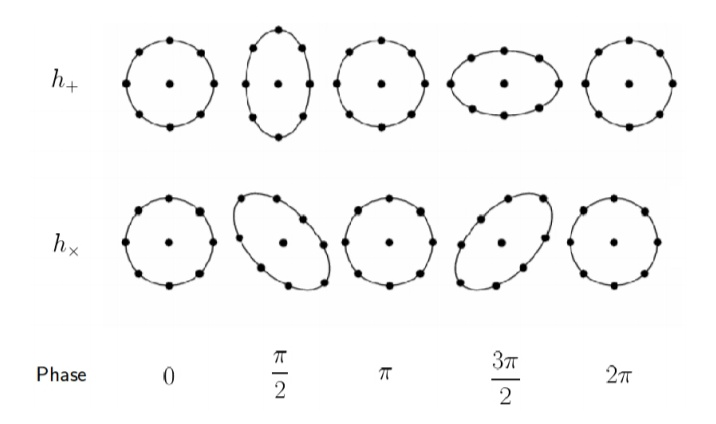
\includegraphics[scale=0.4]{images.tex/effect_of_gw.jpeg}
    \caption{Shape of the object when gravitational wave passes through it when the phase difference of wave changes by $\pi/2$.\\
    \textbf{Source :-} Wavelet graphs for the detection of gravitational waves : application to eccentric binary black holes by Philippe Bacon}
\end{figure}

\begin{figure}[h]
    \centering
    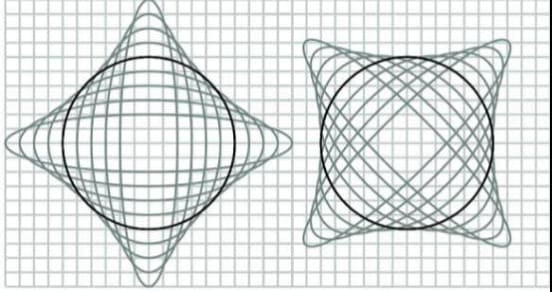
\includegraphics[scale=0.4]{images.tex/polarization.jpeg}
    \caption{Pictorial representation of two Linear polarization of gravitational waves. \\ Source:- \url{https://www.researchgate.net/figure/fig4_228909324}}
\end{figure}

\pagebreak
\subsection{Energy transported by gravitational wave}

When sources produce gravitational waves, their energy is converted to Gravitational waves. Since generally the sources are very massive Energy of gravitational waves will be very large. Since gravitational wave travels in the speed of light, the energy is also transported at that speed. And since Energy flux is equal to the product of Energy and speed, The average energy flux `$E$' is given by

\begin{equation}
    E = \frac{c^{3}}{16\pi G} \left \langle (h_{+})^{2} + (h_{\times})^{2} \right \rangle 
\end{equation}

So we see the energy flux is very huge because of the term $\frac{c^{3}}{16 \pi G}$ which is in the order of $10^{33}$ Joules sec/ metre$^2$  and it also depends on the average of the square of the plus and cross polarized amplitudes `$h_{+}$' and `$h_{\times}$'. \\

Due to such huge energy it carries the wave can travel unimpeded forever through space and no obstacle can damp gravitational wave because the space in which the obstacle lies itself is the medium of the wave. But the Doppler effect and decrease in amplitude due to radiation of energy causes the wave to die out after the wave travels a very long distance according to the relation $Amplitude \propto \frac{1}{r}$\:. 
\\

\noindent So the power or intensity of gravitational wave decreases as it moves through space according to this inverse square law i.e. as the wave moves in space through a distance `$r$' The energy of wave will be spread-out in space across a sphere of radius`$r$' through Surface area of sphere $4\pi r^2$. Since the intensity of wave is Energy over time, Intensity reduces as $r^2$

\begin{equation*}
    E_{flux}= \frac{Energy}{Area} = \frac{E}{4\pi r^2}
\end{equation*}

\begin{equation*}
    E_{flux} \propto \frac{1}{r^2}
\end{equation*}

\noindent But since $E_{flux} \propto Amplitude^2$ we get the relation that $Amplitude \propto \frac{1}{r}$. i.e Amplitude decreases as distance from source increases. 

\begin{figure}[h]
    \centering
    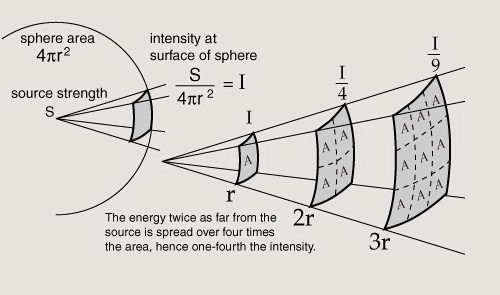
\includegraphics[scale=1]{images.tex/inverse_square.jpeg}
    \caption{ Here we see how the intensity of wave changes as it goes farther from the source according to the inverse square law.\\
    \textbf{Source :-} \url{http://www.mysearch.org.uk/website1/html/339.Laws.html}}
\end{figure}

\pagebreak
wirte similarities and differences between EM and GW

\pagebreak


\section{Sources of Gravitational waves}
Theory of general relativity predicts that gravitational waves can be generated by any dynamically changing system containing moving objects by producing radiation-reaction forces in their source i.e. waves will be generated and carries the exact rate of energy which is extracted from the source. 

Gravitational waves can be produced by an object which is accelerating or a Binary revolving system, merging black holes, neutron star collisions, primordial black holes, etc. But one common nature is all these objects is, they change the curvature of space-time. Thus radiate waves. 
 
\subsection{Single accelerating object in space}
 Accelerating objects like pulsars can create gravitational wave. According to general relativity, mass creates stress in space-time and thus can change the geometry of it by bending and changing the curvature. Then if this object moves, then the curvature also moves along with it. But if the object accelerates in space-time in a circular manner, then the ripples will be created in space-time which is which radiates gravitational waves. This is similar to creation of water waves when we move our finger in a circular fashion in water. So higher the mass of object and it's acceleration, stronger is the gravitational wave it produces.
 
 Such continuously spinning bodies produces continuous gravitational waves, where it's nature is sinusoidal for a longer period of time. This happens only if spin rate of this object is constant. Such gravitational waves have same frequency and amplitude. Such types of gravitational waves are not yet discovered.\\


\begin{figure}[h]
    \centering
    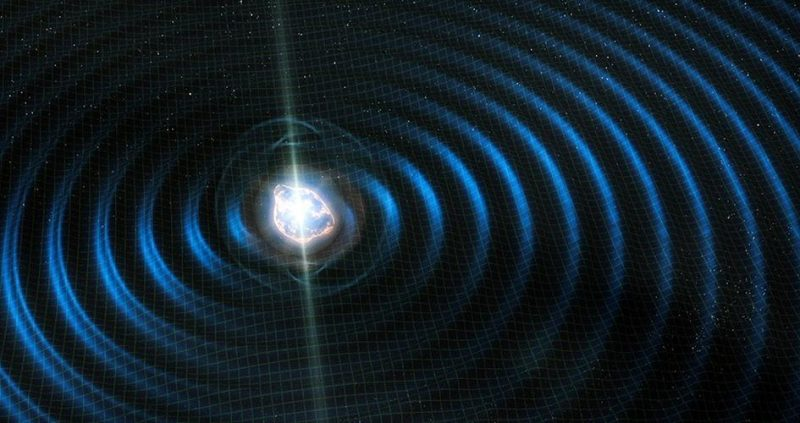
\includegraphics[scale = 0.33]{images.tex/continuous_gw.jpg}
    \caption{Computer simulation of Continuous gravitational wave by a pulsar. \\
    \textbf{Source :-} \url{https://earthsky.org/space/}}
\end{figure}

\begin{figure}[h]
    \centering
    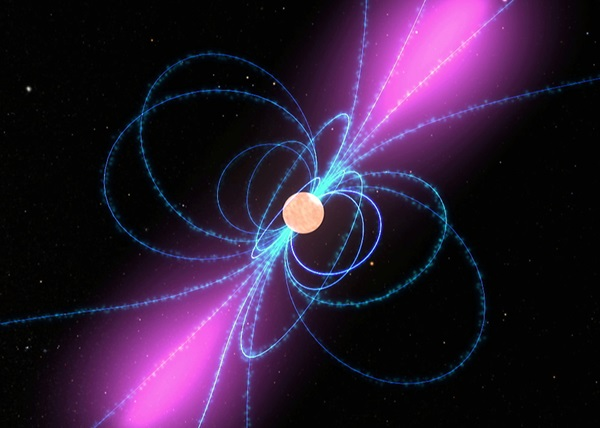
\includegraphics[scale = 0.33]{images.tex/pulsar.jpg}
    \caption{A rotating pulsar.   \textbf{Source}:- \url{https://astronomy.com/news/2018/02/}}
\end{figure}

\pagebreak
\subsection{Revolving Binary Systems}

Revolving binary systems are a very high energy systems which are formed when two massive objects orbit around their common centre of mass called barycenter. Average total mass of such systems are usually greater than 30 solar masses. And average loss of energy per second by such systems will be every huge which will be converted to gravitational waves. Such systems create gravitational waves by a mechanism called `Inspiral'. There are four phases in this mechanism. \\

\textbf{Interlocking phase} :- This the longest phase where the bodies come closer and get interlocked by their gravity and start to revolve each other around the barycentre. \\

\textbf{Spiral phase} :- Here the objects start getting close as they revolve. Due to the decrease in the distance between them the orbital energy is decreased and this energy is radiated as gravitational wave. But as they come closer and closer, they loose more and more energy, thus the intensity of gravitational wave increases.\\

\textbf{Merger phase} :- During this phase, the bodies collide by producing immense gravitational waves and merge. \\

\textbf{Ring-down phase} :- Finally, the merged bodies become stable and the gravitational wave intensity decreases exponentially and they stop producing gravitational waves. \\

Revolving binary systems produce compact binary inspiral gravitational waves. This is because the intensity of gravitational waves increases slowly during interlocking phase, and exponentially during the spiral phase, then it reaches a peak in merger phase, and finally it decreases rapidly to zero during ring-down phase. The detectors are capable of recording the signal only for a small range of frequency, So in this wave form, the frequency comes to the detecting range and rapidly goes out of range. Thus the signal strength suddenly increases and stops.

\begin{figure}[h]
    \centering
    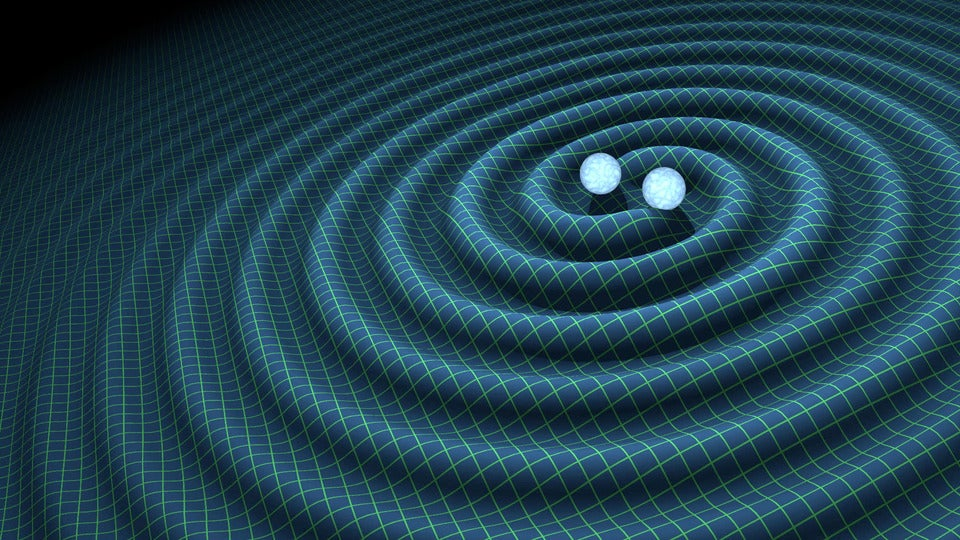
\includegraphics[scale=0.45]{images.tex/binaries.jpeg}
    \caption{Two massive bodies in inspiral mechanism creating gravitational waves \\
    \textbf{Source :-} https://www.scientificamerican.com/article/gravitational-waves-discovered-from-colliding-black-holes1/}
\end{figure}

\pagebreak

\subsubsection{Binary Black Holes (BBH)}

Black holes are massive objects that can warp space-time extensively. If two black holes get closer and start the inspiral mechanism ,they create ripples in space-time and radiate gravitational waves. Such gravitational waves were the first ones to be detected by LIGO in 2015, September 14th. It was estimated that the collision occurred 1.3 billion years ago, thus the merger occurred 1.3 billion light-years away. This merger was named as `\textbf{GW150914}' meaning Gravitational Wave on 15/09/14. This signal lasted for about half a second.

\subsubsection{Binary Neutron Stars (BNS)}

Neutron stars are dense stars formed by the remnants when a massive star explodes as Supernova. So when two neutron stars merge through inspiral mechanism, they can radiate gravitational waves. First BNS merger was detected on 17th August 2017 and this was named as `\textbf{GW170817}', where the merger was analyzed both by Electromagnetic waves (Gamma ray) and gravitational waves. The signal lasted for comparatively longer duration for about 100 seconds, thus the mass was estimated to be lesser than black holes and was recognised as neutron star merge.



\begin{figure}[h]
    \centering
    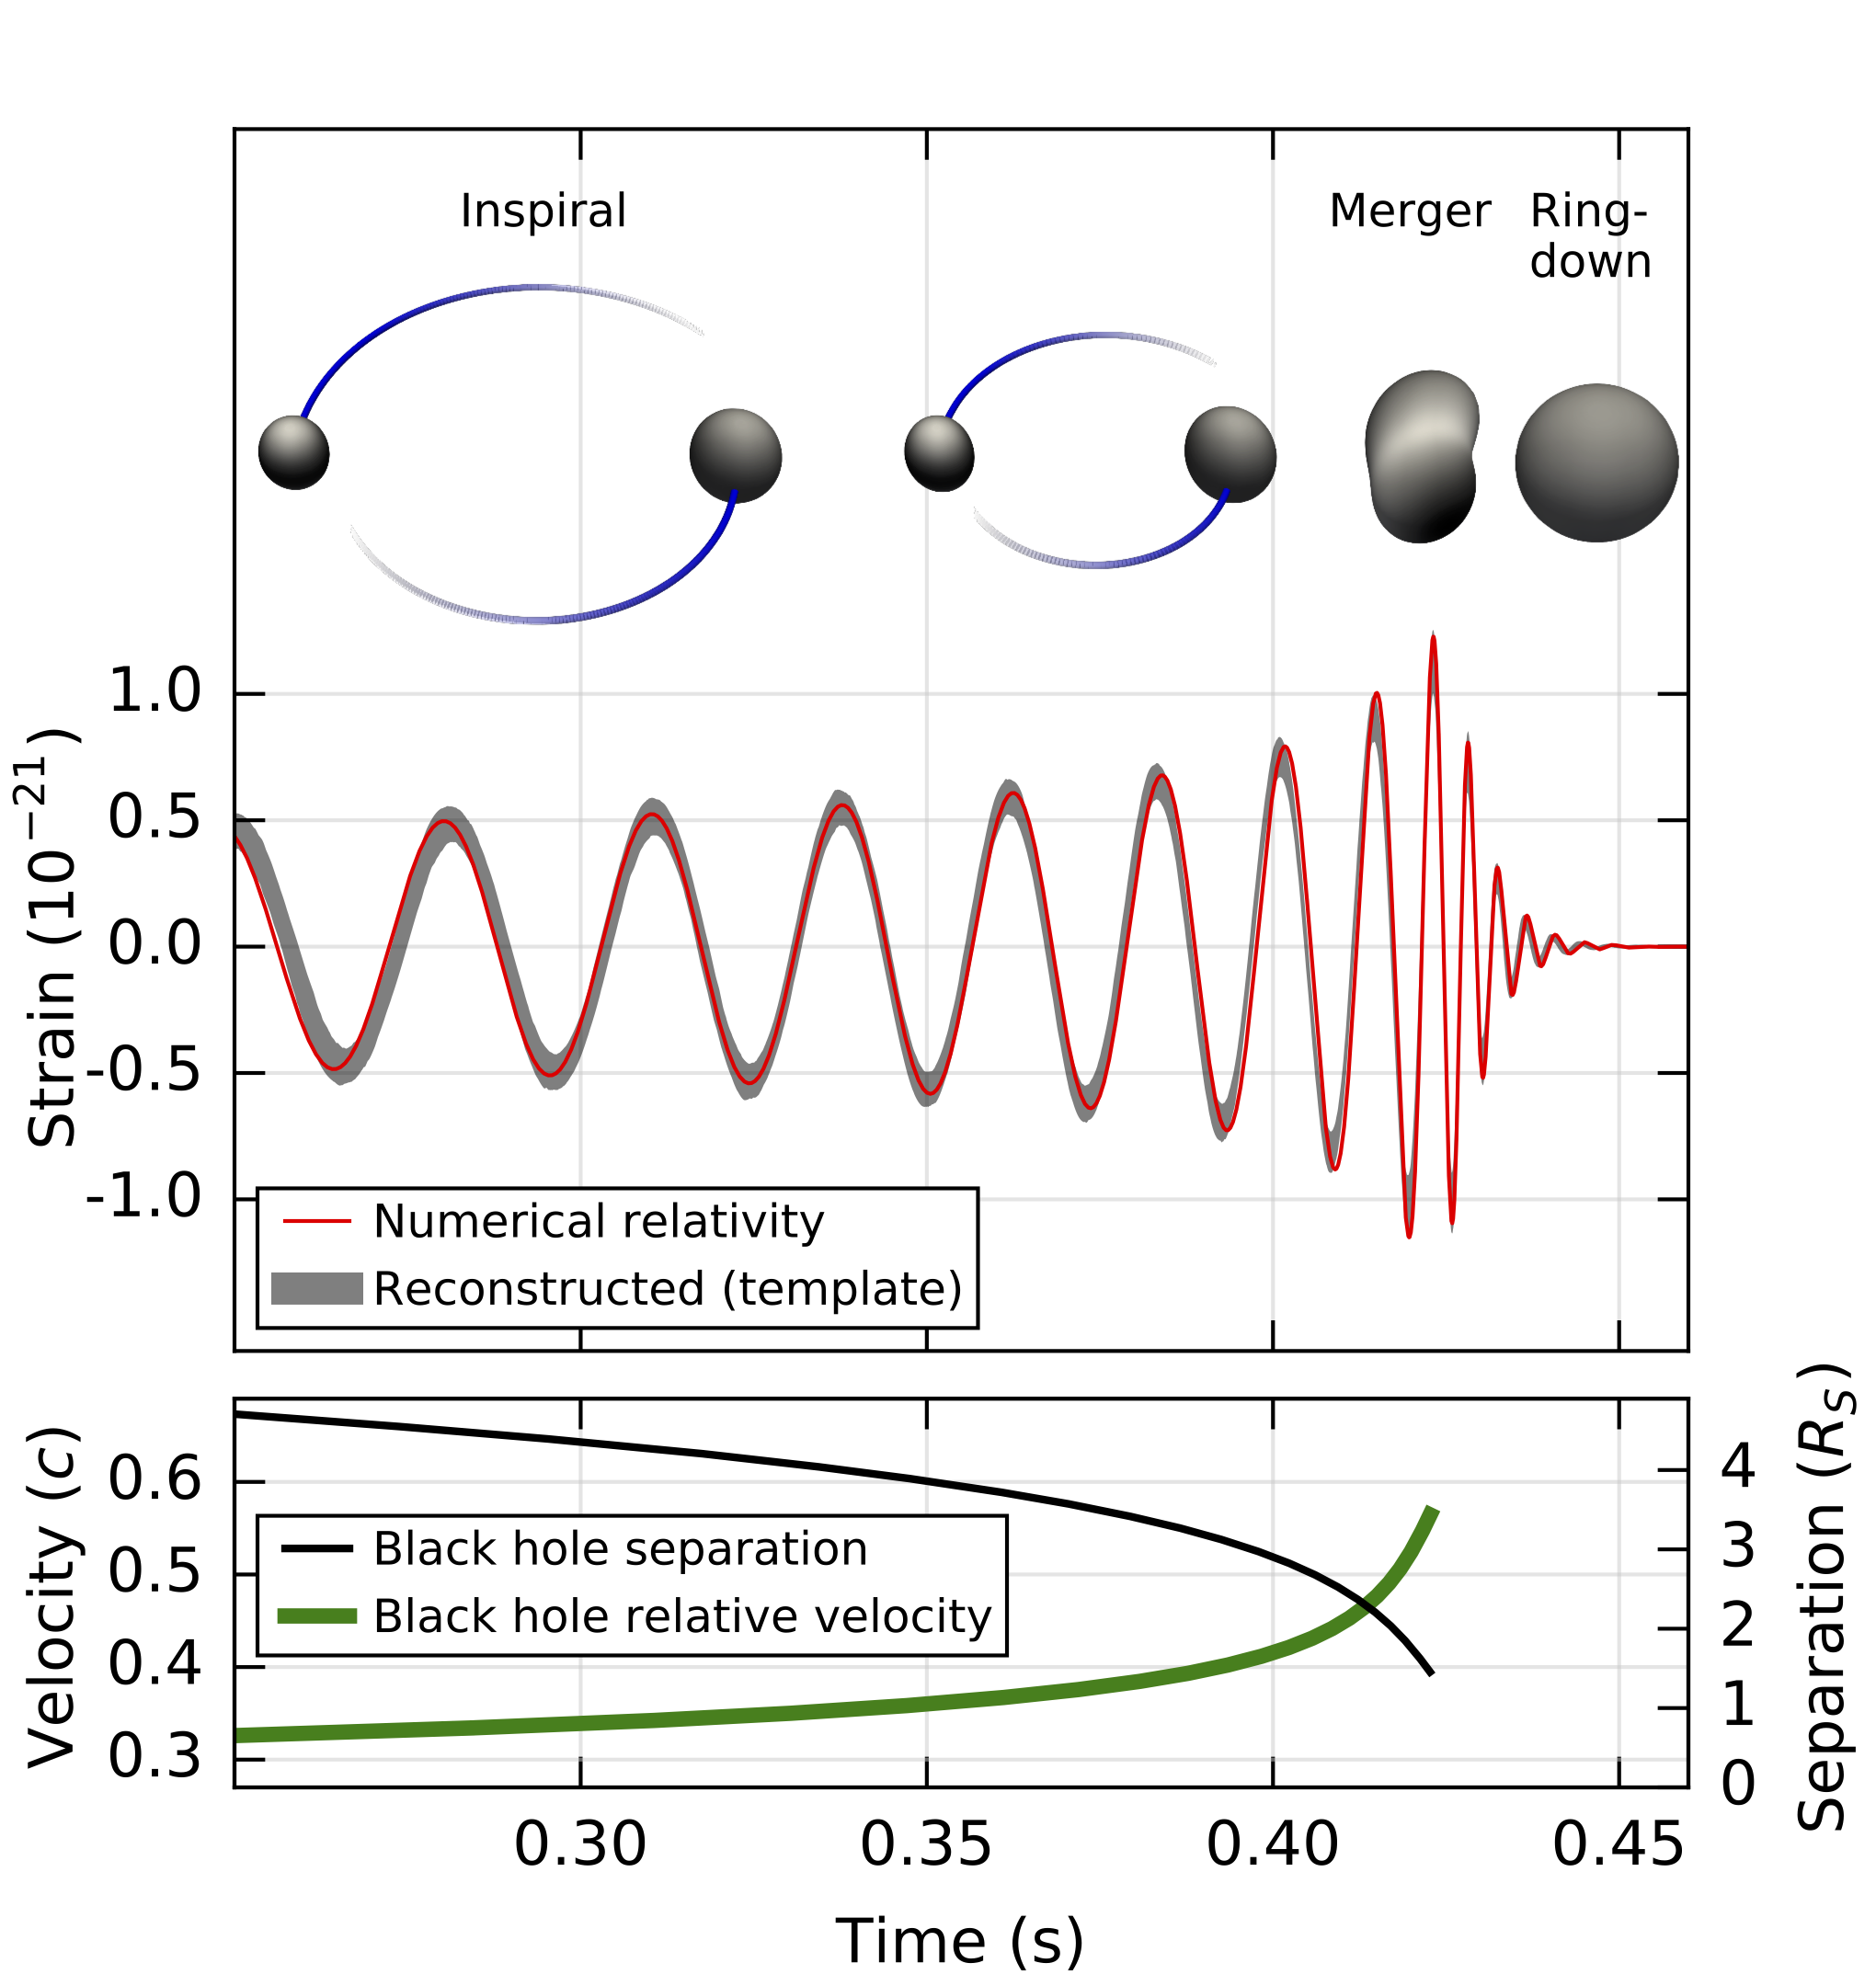
\includegraphics[height = 7cm, width = 8 cm]{images.tex/GW150914.png}
    \caption{Characteristics of GW150914   Source:-\url{https://www.ligo.org/science/}}
\end{figure}

\begin{figure}[h]
     \centering
     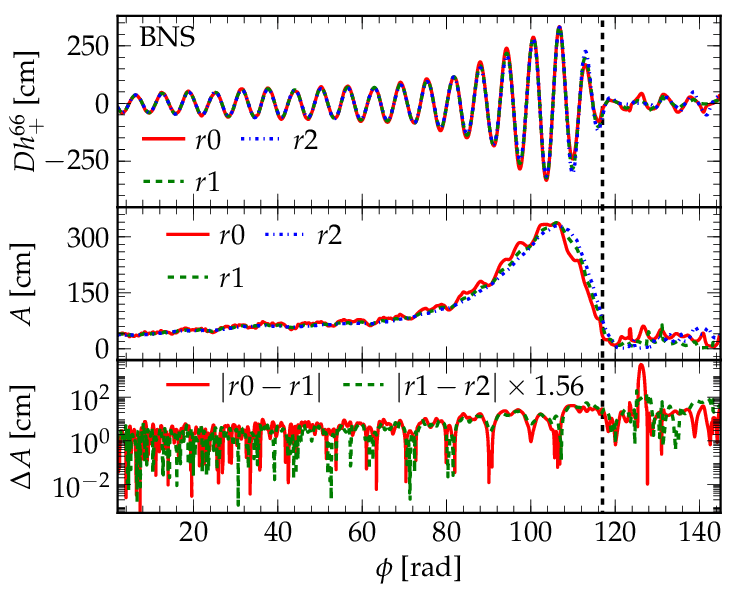
\includegraphics[scale = 0.3]{images.tex/GW170817.png}
     \caption{Characteristics of GW170817\\ Source:- \url{https://www.researchgate.net/publication/233846764}}
\end{figure}

\pagebreak






























































\pagebreak















































































\pagebreak

\section{Types of Gravitational Waves}
\hspace{0.6 cm} Gravitational waves are produced by each and every body which is accelerating, for e.g. moving cars, air planes, humans, etc. However, they are too small to be noticed and detected with our current technology. In order to study gravitational waves, we need to look at object which are massive and much more bigger than our own solar system like black holes, neutron stars, or huge stars at the end of their lives like gamma ray bursts, pulsars, orbiting black holes, rapidly spinning neutron stars, etc. In fact our universe is filled with many such objects which produce gravitational waves with a significant amplitude and energy. This section was referred by \cite{Allen1996TheSG}, \cite{Neutron_wiki}, \cite{Linear}, \cite{sounds_of_space} \\

\noindent Gravitational wave sources have been divided into following categories:-

\begin{enumerate}
    \item \textbf{Short duration sources :-} Compact binary coalescence, supernovae, gamma ray burst.

    \item \textbf{Continuous sources :-} Pulsars, magnetars, rapidly spinning neutron stars, low mass X Ray binaries, super massive black hole binaries.

    \item \textbf{Stochastic sources :-} Metric fluctuations generated in the very early universe.
\end{enumerate}

\noindent To understand gravitational waves better, LIGO scientists have divided the waves in four categories. The division of the gravitational waves is based on their sources and their characteristic vibration as detected by the interferometers.  They are divided into Continuous, Compact Binary Inspiral, Stochastic and Burst Gravitational waves.

\begin{enumerate}

\item \textbf{Continuous Gravitational Waves} 
    
\noindent Such Gravitational Waves are produced by objects that have constant frequencies and amplitude like a single spinning neutron star. Neutron stars are basically a result of the supernova explosion of a massive star, combined with gravitational collapse, that compresses the core so much that the star density becomes as that of atomic nuclei. Radius of neutron stars will be in the order of 10 kilometers, and mass will be around 1.4 Solar masses. So density will be around $10^{17}\: \text{Kg}\text{m}^{-3}$. The properties of the gravitational waves depend on the spin rate of the star. Therefore, if the spin rate is constant, the properties of gravitational waves (frequency and amplitude) will also remain constant i.e. \textit{continuous}. Spinning neutron stars that possess asymmetric deformations or imperfections in their space produce gravitational waves as it swiftly rotates about its axis. The reasons or effects which can produce asymmetry could be Accretion (large mountain), Magnetic deformations or Pulsar glitches.

\vspace{0.2cm}

\item \textbf{Compact Binary Inspiral Gravitational Waves}
    
\noindent Most of the waves detected so far by LIGO are part of this category. Compact Binary In spiral Gravitational Waves are formed by orbiting pairs of massive objects like neutron stars or black holes. There are three kinds of systems in this category of gravitational wave generators where each one has different characteristics. They are Binary Black Hole system (BBH), Binary Neutron Star system (BNS) and Black Hole-Neutron Star binary system (BHNS). The main phases involved in such systems are spiral, merger and ring-down.

\vspace{1mm}
Let us start by considering two black holes orbiting each other. Initially they are widely separated, spiral occurs over millennia, with each revolution, they emit very weak gravitational waves. Slowly as the energy is lost from the system in the form of gravitational waves, the binary is thus pushed into an orbit with smaller radius and higher orbital frequency. Thus the distance between them decreases and their speeds increase. This causes the frequency of the gravitational waves to increase. Now comes the Merger stage where the black holes come very close and are about to collide to form a single black hole and the black hole thus formed has large distortions in its shape. The strongest gravitational waves are emitted during this process. The distortions thus formed are radiated away as more gravitational waves during the ring-down phase and an undistorted but rotating black hole is left behind. Due to the increase in frequency, the pitch also increases and as a result these gravitational waves would produce a chirp sound. Current results indicate that compact binary objects may well be the most promising sources of gravitational waves rather than supernova collapse.

\item \textbf{Stochastic Gravitational Waves}

These types of waves are generated from random sources, typically arising from a large number of unresolved and uncorrelated events and thus they are the most difficult gravitational waves to detect. Stochastic Gravitational Waves are believed to be the result of processes that took place shortly after the big bang. Just like the Cosmic Micro-wave Background (CMB), these gravitational waves arise from a large number of independent, random events merging to create a cosmic gravitational wave background. Due to their random motion, these waves are the most smallest, that's why the final signal has stochastic nature and the difficult to detect with our current technology. These waves may be analyzed statistically but they cannot be predicted precisely. Detecting these gravitational waves from the Big Bang could allow us to see back in the history of the Universe.

\vspace{0.2cm}

\item \textbf{Burst Gravitational Waves}   

Of all the types of gravitational waves, these waves come from the sources which are yet to be known and thus the form of waves which will be produced is also unexpected. Burst gravitational waves come from short-duration unknown sources. Since we are unfamiliar with these sources, thus its modelling is a big challenge since these will not have well defined properties which are known earlier to us like those of compact binary inspiral waves. Some believe that these waves are produced from systems like supernovae. They are believed to have a 'pop' and 'crack' sound. However, it is difficult to say anything as of now due to the lack of knowledge about their origin. But if we discover an efficient way to detect such GW, revolutionary information about the universe could be revealed.

\end{enumerate}

\begin{figure}[h]
    \centering
    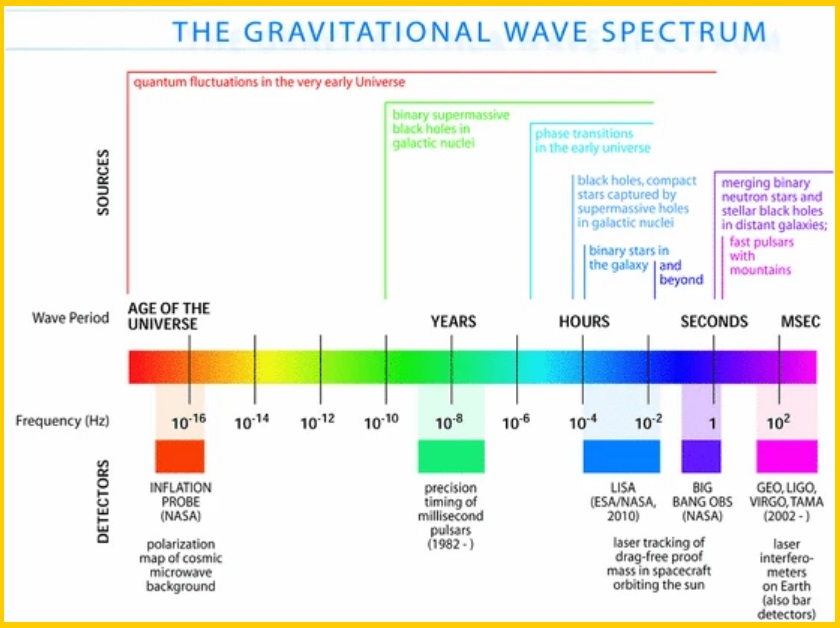
\includegraphics[scale=0.6]{images.tex/Stochastic_gw.jpg}
    \caption{Gravitational Wave Spectrum. Source :- \href{https://link.springer.com/article/10.1007/s41114-017-0004-1}{Detection methods for stochastic gravitational-wave backgrounds by Joseph D. Romano}}
\end{figure}

\begin{figure}[h]
    \centering
    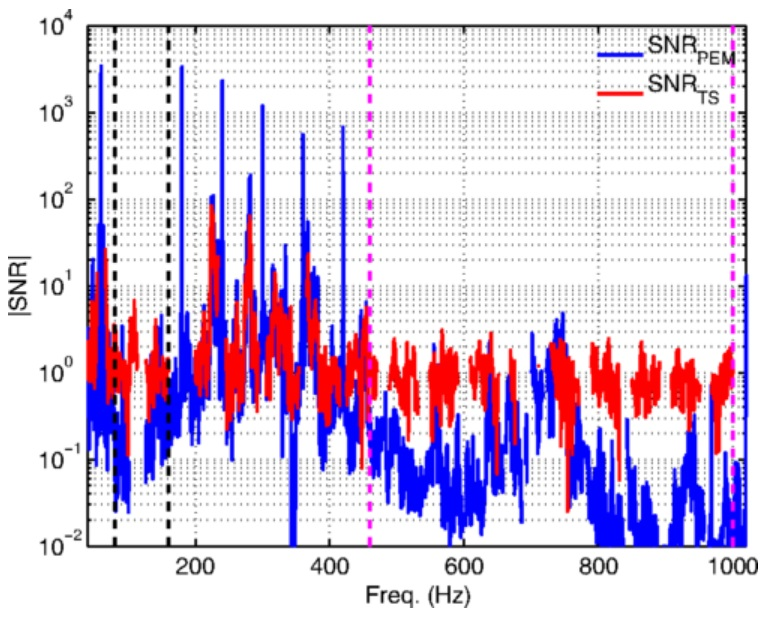
\includegraphics[height = 3.5 cm, width = 10cm]{images.tex/Stochastic wave form.jpg}
    \caption{Stochastic gravitational wave form.\, Source :- \href{https://journals.aps.org/prd/abstract/10.1103/PhysRevD.91.022003}{Searching for stochastic gravitational waves using data from the two co-located LIGO Hanford detectors by J. Aasi}}
\end{figure}

\pagebreak



















































\pagebreak

\section{Why study Gravitational Waves}
\hspace{1cm}Gravitational waves are already used as an important member of multi-messenger astronomy and these can be used to study in depth many objects or phenomena such as:

\begin{itemize}

\item Cataclysmic variables
\item Binary Neutron Stars
\item Young Neutron Stars (the r-mode instability)
\item Low-mass X-ray binaries
\item CMB and Galaxy formation

\end{itemize}

\hspace{1cm}Gravitational waves are emitted by the masses and sent as ripples across spacetime which is completely different from the mechanism of production and transmission of EM waves. Therefore, it could give us more information on the subject matter at hand.

\hspace{1cm}Gravitational waves provide further information about black holes that would otherwise be invisible. Gravitational waves also weakly interact with matter (apart from lensing), thereby reducing energy lost or scattered before reaching the detector. This implies better understanding of inconspicuous regions of space, like the interior of a supernova or the Big Bang.

\subsection{Uses of their Detection}

\hspace{1cm} Gravitational Waves are also used in Astronomy because it allows us to observe the universe the universe in a different way, providing us information about matter such as:

\subsubsection{Information about the Big Bang}
\hspace{1cm}Gravitational waves have travelled almost unimpeded through the universe since they were generated (which happened $10^{-24}$s after the Big Bang, far earlier than the CMB radiation). Possibilities of non-inflation mechanisms that produce gravitational waves are high. One such possibility could be cosmic strings, which ought to be detectable using gravitational waves. LIGO/VIRGO observations of compact binary in spiral have the potential to bring us far more information than just binary masses and spins:

\subsubsection{Test the theory of General Relativity}
\hspace{1cm}They can be used for high-precision tests of general relativity. Radiation reaction to some scalar waves in scalar-tensor theories has a signature that can be found with high precision in LIGO/VIRGO.

\subsubsection{Detection of the Hubble Constant}
\hspace{1cm}They can be used to measure the Universe’s Hubble constant, deceleration parameter, and cosmological constant.Gravitational waves bring a new window to validate the general theory of relativity and cosmological constant as the correct explanation of the theory of gravity and cosmic acceleration. Hubble's Constant shows the expansion of the Universe by showing how distant galaxies are moving away from us and is given by:
 
\begin{equation}
v = H_o*d
\end{equation}

where, v is the Velocity of a galaxy, in $kms^{-1}$

      $H_{o}$ is the Hubble Constant, measured in $kms^{-1}Mpc^{-1}$
      
      d is the Distance of a galaxy, in Mpc


\vspace{1cm}
\begin{figure}
    \centering
    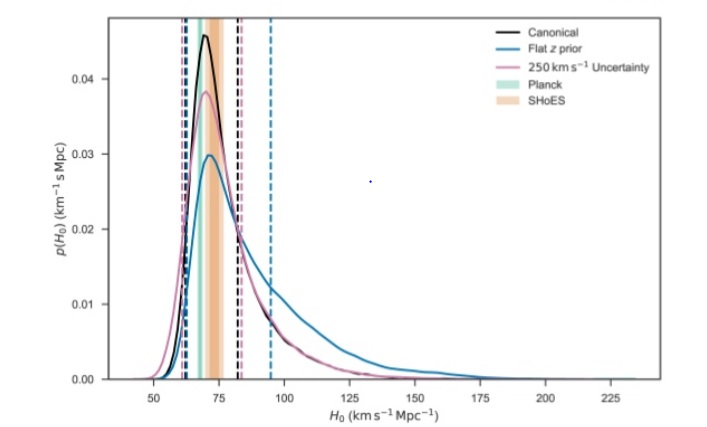
\includegraphics[scale=0.75]{images.tex/HCGW.jpg}
    \caption{Hubble's Constant using Gravitational waves. Source: \url{https://www.researchgate.net/profile/Michael-Ross-9/publication/324600496}}
\end{figure}
\subsubsection{Polarization of Gravitational Waves}
\hspace{1cm}Gravitational waves carry 2 independent polarizations. A wave will usually have a combination of both. Some sources (rotating) will emit both polarizations with some lag between them. Studying this would give the nature of the source and its rotation.


\subsubsection{Centrifuge of Binary Stars}
\hspace{1cm}A more careful calculation shows that, for unequal masses, the quadrupole amplitude and the rate of shrinking depend on the masses only through the combination:
\begin{equation}
\ M=\mu^{3/5}*M^{2/5}\
\end{equation}
\hspace{1cm}This is called the chirp mass, where, $\mu$ is the reduced mass and M the total mass. If one can observe, in gravitational radiation, the shrinking time, then one can infer the chirp mass. If one then measures the amplitude of the radiation, the only unknown is the distance r to the source. Gravitational wave observations of orbits that shrink because of gravitational energy losses can therefore directly determine the distance to the source. This is another way in which gravitational wave observations are
complementary to electromagnetic ones, providing information that is hard to obtain
electromagnetically.

\subsubsection{Spiralling of Black Holes and Neutron Stars}
\hspace{1cm}For a Neutron star or black hole spiralling inwards, the inward spiral has a sort of “map” of it that are emitted in the form of gravitational waves. Analysis of these waves could give information of the body, help determine the type of body(black hole or any other exotic object like a naked singularity)  and can be studied better by LISA for low masses and high frequencies as opposed to LIGO/VIRGO that can capture large masses and low frequencies.


\subsection{Summary}

\hspace{1cm}In summary, we can say gravitational waves provide a new tool for astronomy as well as cosmology and will be ever evolving in terms of types of observations possible ranging from new ways to test for dark matter and the validity general relativity with high precision and observations that simply would not be possible with just electromagnetic waves.This also provides an alternate method to validate the cosmological constant, Hubble’s constant, and various other uses. This section was referred from these 2 papers \cite{Schutz_1999},\cite{Mukherjee_2020}


\section{Indirect Evidences of Gravitational Waves}
















































































\pagebreak

\section{Direct search for Gravitational waves}



















































































\pagebreak
















































































\pagebreak
















































































\pagebreak
















































































\pagebreak

\section{Detection of Gravitational waves using LIGO }
















































































\pagebreak
















































































\pagebreak

\section{Conclusion}
















































































\pagebreak
































































































































































\pagebreak

\printbibliography
\end{document}
